\documentclass[tikz,border=6pt]{standalone}
\usetikzlibrary{arrows.meta,positioning,calc}
\makeatletter
\AtBeginDocument{\global\let\pgf@selectfontorig\relax}
\makeatother

\tikzset{
  nodebox/.style={draw=black, rounded corners=4pt, very thick, fill=gray!4,
    minimum width=10mm, minimum height=7mm, align=center, inner sep=2pt},
  initial/.style={-Latex, very thick},
  edge/.style={-Latex, thick, shorten >=1pt, shorten <=1pt},
  labelbox/.style={fill=white, inner sep=1.2pt, font=\scriptsize},
  aptxt/.style={font=\scriptsize, text=gray!65!black, anchor=north east},
}

\newcommand{\initarrow}[2]{\draw[initial] #1 -- (#2);}
\newcommand{\statelabel}[2]{\node[aptxt] at ($(#1.south east)+(0.02,-0.05)$) {#2};}

% =====================================================================
% Safety -- Variant B:  "Choose A_1 or A_2" non-deterministic controller.
%
%   H = { alpha_{i,1}, alpha_{i,4}  |  i = 1, 2 }
%
%   Safety   : YES.  c_0 nondeterministically selects either A_1 or A_2;
%                    after firing alpha_{i,1} the controller can only
%                    return to c_0 via the matching alpha_{i,4}, so a
%                    second light cannot start before the first finishes.
%
%   Liveness : NO.   alpha_{3,1} is not in the controller's alphabet,
%                    so A_3 never leaves r_3.  An unfair scheduler may
%                    additionally always pick A_1, starving A_2.
% =====================================================================
\begin{document}
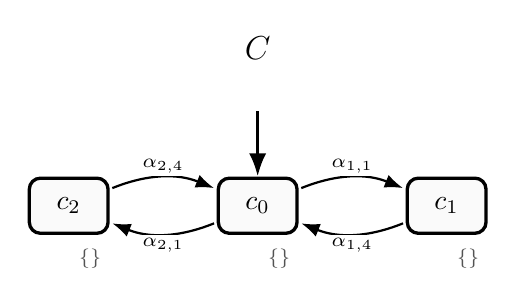
\begin{tikzpicture}[scale=1, transform shape]

  \node[font=\bfseries\large] at (0, 2.0) {$C$};

  \node[nodebox] (b0) at ( 0,    0) {$c_0$};
  \node[nodebox] (b1) at ( 2.4,  0) {$c_1$};
  \node[nodebox] (b2) at (-2.4,  0) {$c_2$};

  \statelabel{b0}{$\{\}$};
  \statelabel{b1}{$\{\}$};
  \statelabel{b2}{$\{\}$};

  \initarrow{(0, 1.2)}{b0.north}

  \draw[edge, bend left=22] (b0) to node[labelbox, above] {$\alpha_{1,1}$} (b1);
  \draw[edge, bend left=22] (b1) to node[labelbox, below] {$\alpha_{1,4}$} (b0);
  \draw[edge, bend left=22] (b0) to node[labelbox, below] {$\alpha_{2,1}$} (b2);
  \draw[edge, bend left=22] (b2) to node[labelbox, above] {$\alpha_{2,4}$} (b0);

\end{tikzpicture}
\end{document}
